\chapter{Iteraciones del PUD}
\label{chap::iteraciones}

Este anexo pretende ofrecer un análisis descriptivo de las diferentes iteraciones por las que ha pasado el presente proyecto durante su desarrollo, siguiendo para ello el \acs{PUD}, como se comentó en la sección \ref{sec::pud}.

A continuación se hará un recorrido por cada iteración, explicando en qué han consistido y detallando la repercusión global de cada una. Las iteraciones están agrupadas en tres fases: Inicio, Elaboración y Construcción.

Cada iteración es detallada desde 2 puntos de vista:

\begin{itemize}
\item {\bf Local}

Con este enfoque se ofrece una descripción de en qué ha consistido la iteración. Además se detalla la proporción del desarrollo general que ha supuesto. Es importante comprender que las cifras de cada iteración no representan la repartición del esfuerzo de esa tarea, sino el porcentaje de cada artefacto que ha sido completado en esa iteración.

\item {\bf Global}

Con este enfoque se muestran los porcentajes completado y restante del desarrollo global, desde el inicio de la primera iteración hasta la finalización de la iteración en cuestión.

\end{itemize}

Al finalizar este anexo se ofrecerá una descripción gráfica de la evolución seguida durante el proceso.

\section{Iteraciones de inicio}

%% ==================================================

\subsection*{Iteración I1}

\begin{itemize}    
\item {\bf Descripción}:

Esta primera iteración se ha basado en la elaboración del análisis de un conjunto inicial de requisitos ---los más importantes--- así como el estudio de casos de uso de una parte de los mismos.

Al mismo tiempo que parte de los requisitos quedaban especificados por completo, una pequeña parte del diseño del software a construir quedaba definido.

Los artefactos que se han visto involucrados en esta iteración son, por lo tanto, el análisis de requisitos, en análisis de casos de uso y el diseño.

Esta iteración ha tenido una duración de 75 horas aproximadamente.
\end{itemize}

\begin{minipage}[c]{0.45\linewidth}
  \begin{itemize}    
  \item {\bf Desarrollo local}:
    \begin{itemize}
    \item Requisitos: 53.6\%.
    \item Casos de uso: 27.8\%.
    \item Diseño: 10\%.
    \item Implementación: 0\%.
    \item Pruebas: 0\%.
    \end{itemize}
  \item {\bf Desarrollo global}: 18.28\%
  \item {\bf Desarrollo restante}: 81.72\%
  \end{itemize}
\end{minipage}
\begin{minipage}[c]{0.45\linewidth}
  \begin{figure}[H]
    \begin{center}
      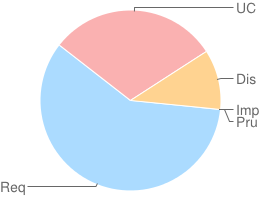
\includegraphics[width=6cm]{images/i1.png}
      % http://charts.hohli.com

      % http://chart.apis.google.com/chart?cht=p&chs=260x200&chd=s:DhPGD&chl=Imp|Req|UC|Dis|Pru&chco=abdbff,fab1b1,ffd391,ffa1fc,b6e0be&chf=bg,s,FFFFFF|c,s,FFFFFF
      \caption{Iteracción I1}
      \label{fig::i1}
    \end{center}
  \end{figure}
\end{minipage}

\section{Iteraciones de elaboración}

%% ==================================================

\subsection*{Iteración E1}

\begin{itemize}    
\item {\bf Descripción}:

Esta primera iteración de la fase de elaboración ha supuesto los primeros pasos de la implementación ---en una proporción modesta---, al tiempo que los análisis de requisitos y de casos de uso han sido ampliados.

Los artefactos que se han visto involucrados en esta iteración son, por lo tanto, el análisis de requisitos, en análisis de casos de uso, el diseño y la implementación.

Esta iteración ha tenido una duración de 50 horas aproximadamente.
\end{itemize}

\begin{minipage}[c]{0.45\linewidth}
  \begin{itemize}    
  \item {\bf Desarrollo local}:
    \begin{itemize}
    \item Requisitos: 17.8\%.
    \item Casos de uso: 22.2\%.
    \item Diseño: 15\%.
    \item Implementación: 5.2\%.
    \item Pruebas: 0\%.
    \end{itemize}
  \item {\bf Desarrollo global}: 30.3\%
  \item {\bf Desarrollo restante}: 69.7\%
  \end{itemize}
\end{minipage}
\begin{minipage}[c]{0.45\linewidth}
  \begin{figure}[H]
    \begin{center}
      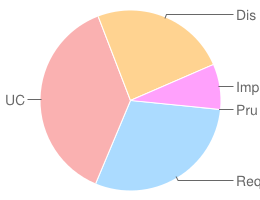
\includegraphics[width=6cm]{images/e1.png}
      % http://charts.hohli.com

      % http://chart.apis.google.com/chart?cht=p&chs=260x200&chd=s:DhPGD&chl=Imp|Req|UC|Dis|Pru&chco=abdbff,fab1b1,ffd391,ffa1fc,b6e0be&chf=bg,s,FFFFFF|c,s,FFFFFF
      \caption{Iteracción E1}
      \label{fig::e1}
    \end{center}
  \end{figure}
\end{minipage}

%% ==================================================

\subsection*{Iteración E2}

\begin{itemize}    
\item {\bf Descripción}:

Esta última etapa de la fase de Elaboración ha supuesto un pequeño avance generalizado. La mayor parte de los esfuerzos se han dedicado al diseño del software. Además se han creado las primeras pruebas unitarias.

Todos los artefactos se han visto involucrados en esta iteración: el análisis de requisitos, en análisis de casos de uso, el diseño, la implementación y las pruebas.

Esta iteración ha tenido una duración de 50 horas aproximadamente.
\end{itemize}

\begin{minipage}[c]{0.45\linewidth}
  \begin{itemize}    
  \item {\bf Desarrollo local}:
    \begin{itemize}
    \item Requisitos: 14.3\%.
    \item Casos de uso: 27.8\%.
    \item Diseño: 50\%.
    \item Implementación: 12.1\%.
    \item Pruebas: 5\%.
    \end{itemize}
  \item {\bf Desarrollo global}: 52.2\%
  \item {\bf Desarrollo restante}: 47.8\%
  \end{itemize}
\end{minipage}
\begin{minipage}[c]{0.45\linewidth}
  \begin{figure}[H]
    \begin{center}
      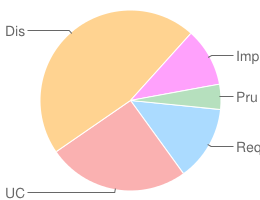
\includegraphics[width=6cm]{images/e2.png}
      % http://charts.hohli.com

      % http://chart.apis.google.com/chart?cht=p&chs=260x200&chd=s:DhPGD&chl=Imp|Req|UC|Dis|Pru&chco=abdbff,fab1b1,ffd391,ffa1fc,b6e0be&chf=bg,s,FFFFFF|c,s,FFFFFF
      \caption{Iteracción E2}
      \label{fig::e2}
    \end{center}
  \end{figure}
\end{minipage}


\section{Iteraciones de construcción}

\subsection*{Iteración C1}

\begin{itemize}    
\item {\bf Descripción}:

En esta iteración se ha realizado un pequeño esfuerzo por prácticamente terminar de definir los casos de uso. Dado que en la etapa de construcción el objetivo es centrarse en la implementación, en esta primera iteración se ha pretendido dejar prácticamente finalizados los artefactos previos a la misma.

En esta iteración están implicados todos los artefactos: análisis de requisitos, en análisis de casos de uso, diseño, implementación y pruebas.

Esta iteración ha tenido una duración de 75 horas aproximadamente.
\end{itemize}

\begin{minipage}[c]{0.45\linewidth}
  \begin{itemize}    
  \item {\bf Desarrollo local}:
    \begin{itemize}
    \item Requisitos: 3.6\%.
    \item Casos de uso: 16.6\%.
    \item Diseño: 5\%.
    \item Implementación: 2.9\%.
    \item Pruebas: 5\%.
    \end{itemize}
  \item {\bf Desarrollo global}: 58.8\%
  \item {\bf Desarrollo restante}: 41.2\%
  \end{itemize}
\end{minipage}
\begin{minipage}[c]{0.45\linewidth}
  \begin{figure}[H]
    \begin{center}
      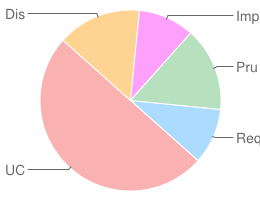
\includegraphics[width=6cm]{images/c1.png}
      % http://charts.hohli.com

      % http://chart.apis.google.com/chart?cht=p&chs=260x200&chd=s:DhPGD&chl=Imp|Req|UC|Dis|Pru&chco=abdbff,fab1b1,ffd391,ffa1fc,b6e0be&chf=bg,s,FFFFFF|c,s,FFFFFF
      \caption{Iteracción C1}
      \label{fig::c1}
    \end{center}
  \end{figure}
\end{minipage}

\subsection*{Iteración C2}

\begin{itemize}    
\item {\bf Descripción}:

Una vez el proyecto se ha centrado en la etapa de construcción, en esta iteración se realiza un gran avance en la implementación del sistema software. El análisis de requisitos queda prácticamente terminado, a excepción de algún pequeño detalle ---requisitos sencillos que surgieron a medida que el desarrollo avanzaba---, y el análisis de casos de uso se finaliza por completo.

En esta iteración están implicados todos los artefactos: análisis de requisitos, en análisis de casos de uso, diseño, implementación y pruebas, con un peso muy importante para la implementación.

Esta iteración ha tenido una duración de 125 horas aproximadamente.
\end{itemize}

\begin{minipage}[c]{0.45\linewidth}
  \begin{itemize}    
  \item {\bf Desarrollo local}:
    \begin{itemize}
    \item Requisitos: 7.1\%.
    \item Casos de uso: 5.6\%.
    \item Diseño: 5\%.
    \item Implementación: 30.6\%.
    \item Pruebas: 23.4\%.
    \end{itemize}
  \item {\bf Desarrollo global}: 73.1\%
  \item {\bf Desarrollo restante}: 26.9\%
  \end{itemize}
\end{minipage}
\begin{minipage}[c]{0.45\linewidth}
  \begin{figure}[H]
    \begin{center}
      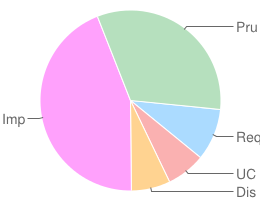
\includegraphics[width=6cm]{images/c2.png}
      % http://charts.hohli.com

      % http://chart.apis.google.com/chart?cht=p&chs=260x200&chd=s:DhPGD&chl=Imp|Req|UC|Dis|Pru&chco=abdbff,fab1b1,ffd391,ffa1fc,b6e0be&chf=bg,s,FFFFFF|c,s,FFFFFF
      \caption{Iteracción C2}
      \label{fig::c2}
    \end{center}
  \end{figure}
\end{minipage}

\subsection*{Iteración C3}

\begin{itemize}    
\item {\bf Descripción}:

Continuando con un esfuerzo mayor para la implementación, esta iteración pretende además avanzar de forma importante con el diseño. Las pruebas son mejoradas y ampliadas.

En esta iteración están implicados los artefactos de análisis de requisitos, diseño, implementación y pruebas, con un peso muy importante, como ya se ha mencionado, para las pruebas.

Esta iteración ha tenido una duración de 80 horas aproximadamente.
\end{itemize}

\begin{minipage}[c]{0.45\linewidth}
  \begin{itemize}    
  \item {\bf Desarrollo local}:
    \begin{itemize}
    \item Requisitos: 3.6\%.
    \item Casos de uso: 0\%.
    \item Diseño: 15\%.
    \item Implementación: 12.3\%.
    \item Pruebas: 25.7\%.
    \end{itemize}
  \item {\bf Desarrollo global}: 82.4\%
  \item {\bf Desarrollo restante}: 17.6\%
  \end{itemize}
\end{minipage}
\begin{minipage}[c]{0.45\linewidth}
  \begin{figure}[H]
    \begin{center}
      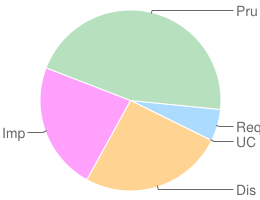
\includegraphics[width=6cm]{images/c3.png}
      % http://charts.hohli.com

      % http://chart.apis.google.com/chart?cht=p&chs=260x200&chd=s:DhPGD&chl=Imp|Req|UC|Dis|Pru&chco=abdbff,fab1b1,ffd391,ffa1fc,b6e0be&chf=bg,s,FFFFFF|c,s,FFFFFF
      \caption{Iteracción C3}
      \label{fig::c3}
    \end{center}
  \end{figure}
\end{minipage}

\subsection*{Iteración C4}

\begin{itemize}    
\item {\bf Descripción}:

En esta última iteración de la fase de construcción los artefactos protagonistas son la implementación y las pruebas. Los análisis de requisitos y de casos de uso quedaron finalizados. El diseño queda en una fase muy avanzada, a falta de pulir pequeños detalles.

En esta iteración están implicados los artefactos de diseño, implementación y pruebas.

Esta iteración ha tenido una duración de 70 horas aproximadamente.
\end{itemize}

\begin{minipage}[c]{0.45\linewidth}
  \begin{itemize}    
  \item {\bf Desarrollo local}:
    \begin{itemize}
    \item Requisitos: 0\%.
    \item Casos de uso: 0\%.
    \item Diseño: 5\%.
    \item Implementación: 11.9\%.
    \item Pruebas: 11.9\%.
    \end{itemize}
  \item {\bf Desarrollo global}: 88.2\%
  \item {\bf Desarrollo restante}: 11.8\%
  \end{itemize}
\end{minipage}
\begin{minipage}[c]{0.45\linewidth}
  \begin{figure}[H]
    \begin{center}
      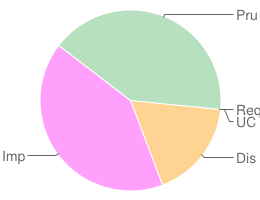
\includegraphics[width=6cm]{images/c4.png}
      % http://charts.hohli.com

      % http://chart.apis.google.com/chart?cht=p&chs=260x200&chd=s:DhPGD&chl=Imp|Req|UC|Dis|Pru&chco=abdbff,fab1b1,ffd391,ffa1fc,b6e0be&chf=bg,s,FFFFFF|c,s,FFFFFF
      \caption{Iteracción C4}
      \label{fig::c4}
    \end{center}
  \end{figure}
\end{minipage}

\section{Etapa de transición}

La etapa de transición del desarrollo de BreakBrain no ha sido abarcada en este documento. Se espera completarla como plan de futuro. Actualmente el proyecto se encuentra en una fase avanzada, pero a falta de terminar algunos detalles antes de poder ponerlo a disposición de los usuarios.

\section{Visión gráfica}

A continuación se representa gráficamente la proporción de desarrollo de cada artefacto software en cada una de las iteraciones. Nótese la clara relación con la figura \ref{fig::pud}, en la que se mostraba la evolución teórica de dichos artefactos según el \acs{PUD}.

% http://chart.apis.google.com/chart?chxl=0:|I1|E1|E2|C1|C2|C3|C4|1:|100|75|50|25|0&chxp=0,1,2,3,4,5,6,7&chxr=0,0,7|1,0,90&chxs=0,676767,11.167,0,l,676767|1,676767,10.833,0,lt,676767&chxt=x,y&chs=700x300&cht=lc&chco=379CF4,00C600,FF9900,0004FF,FF0044&chd=s:AhLJCECA,ARORKDAA,AGJfDDJD,AADHCTIH,AAADDOQH&chdl=An%C3%A1lisis+de+requisitos|Casos+de+uso|Dise%C3%B1o|Implementaci%C3%B3n|Pruebas&chg=0,25&chls=3|2|4.333|3|2&chma=3|0,8

% http://chart.apis.google.com/chart?chxl=0:|I1|E1|E2|C1|C2|C3|C4|1:|0%25|10%25|20%25|30%25|40%25|50%25|60%25|70%25|80%25|90%25|100%25&chxp=0,1,2,3,4,5,6,7|1,0,10,20,30,40,50,60,70,80,90,100&chxr=0,0,7&chxs=0,676767,11.167,0,lt,676767|1,676767,11.167,-0.333,lt,676767&chxt=x,y&chs=700x300&cht=lc&chco=379CF4,00C600,FF9900,0004FF,FF0044&chd=s:AhLJCECA,ARORKDAA,AGJfDDJD,AADHCTIH,AAADDOQH&chdl=An%C3%A1lisis+de+requisitos|Casos+de+uso|Dise%C3%B1o|Implementaci%C3%B3n|Pruebas&chdlp=b&chls=3|3|3|3|3&chma=5|2,22

\begin{figure}[H]
  \begin{center}
    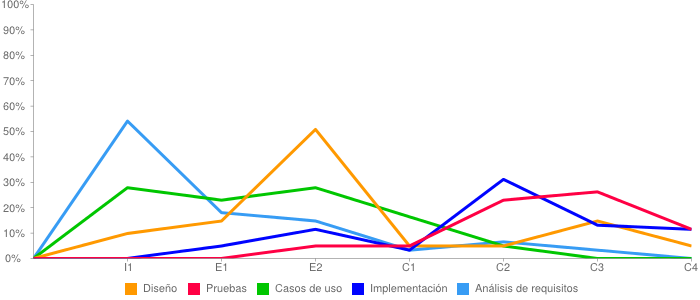
\includegraphics[width=\textwidth]{images/iteraciones.png}
    % http://charts.hohli.com

    % http://chart.apis.google.com/chart?cht=p&chs=260x200&chd=s:DhPGD&chl=Imp|Req|UC|Dis|Pru&chco=abdbff,fab1b1,ffd391,ffa1fc,b6e0be&chf=bg,s,FFFFFF|c,s,FFFFFF
    \caption{Evolución iterativa del desarrollo}
    \label{fig::iteraciones}
  \end{center}
\end{figure}
